% AIAA student-conference paper 2 of 2: the landing algorithm (11-page limit).
% Companion: ../impossibility/main.tex. Shared format: ../aiaa-format.tex.
% Build: latexmk -pdf main.tex   (from this directory)
% Shared format for the two AIAA student-conference papers in this folder (impossibility/ and algorithm/).
% AIAA Meeting Paper (conference) format, reproduced from the published instructions
% ("Preparation of Papers for AIAA Technical Conferences"): letter paper, 1 in margins, Times 10 pt, single column,
% single spaced; title bold 24 pt; abstract bold, indented 0.5 in each side; section headings bold 11 pt, centered,
% Roman numerals; subsections bold flush left with capital letters; sub-subsections italic with arabic numerals;
% captions bold ("Fig. 1" below figures, "Table 1" above tables); footnote symbols; numbered references.
% To use AIAA's own class instead, replace everything between the two "FORMAT" markers by
%     \documentclass[conf]{new-aiaa}  plus the packages and macros marked KEEP,
% and move the title, authors and abstract into that class's \title, \author, \affil and abstract commands.
% ----------------------------------------------------------------------------------------------- FORMAT (begin)
\documentclass[10pt,letterpaper]{article}
\usepackage[margin=1in]{geometry}
\usepackage[T1]{fontenc}
\usepackage{amsmath,amsthm}            % KEEP
\usepackage{txfonts}                   % Times text and math
\usepackage{graphicx,booktabs,array}   % KEEP
\usepackage{enumitem}                  % KEEP
\usepackage{titlesec}
\usepackage[labelfont=bf,textfont=bf,labelsep=quad,justification=centering,skip=6pt]{caption}
\usepackage{lettrine}
\usepackage[numbers,sort&compress]{natbib}
\usepackage[hidelinks]{hyperref}
\urlstyle{same}
\renewcommand{\figurename}{Fig.}
\captionsetup[table]{position=above}
\titleformat{\section}{\normalfont\fontsize{11}{13}\selectfont\bfseries\centering}{\Roman{section}.}{0.5em}{}
\titleformat{\subsection}{\normalfont\normalsize\bfseries}{\Alph{subsection}.}{0.5em}{}
\titleformat{\subsubsection}{\normalfont\normalsize\itshape}{\arabic{subsubsection}.}{0.5em}{}
\titlespacing*{\section}{0pt}{12pt plus 2pt minus 2pt}{6pt}
\titlespacing*{\subsection}{0pt}{9pt plus 2pt minus 1pt}{3pt}
\titlespacing*{\subsubsection}{0pt}{6pt plus 1pt minus 1pt}{2pt}
\renewcommand{\thefootnote}{\fnsymbol{footnote}}
\setlength{\parindent}{0.2in}
\setlength{\parskip}{0pt}
\setlength{\bibsep}{2.5pt}
\renewcommand{\bibfont}{\small}
\makeatletter
\renewcommand{\@biblabel}[1]{[#1]}
\makeatother
\newenvironment{aiaaabstract}{\begin{list}{}{\setlength{\leftmargin}{0.5in}\setlength{\rightmargin}{0.5in}%
  \setlength{\listparindent}{0.2in}\setlength{\itemindent}{0.2in}\setlength{\topsep}{10pt}}\item\bfseries}{\end{list}}
% ------------------------------------------------------------------------------------------------- FORMAT (end)
% KEEP: theorem environments and notation
\newtheoremstyle{aiaa}{4pt}{4pt}{\itshape}{}{\bfseries}{.}{0.5em}{}
\theoremstyle{aiaa}
\newtheorem{theorem}{Theorem}
\newtheorem{lemma}{Lemma}
\newtheorem{proposition}{Proposition}
\newcommand{\norm}[1]{\lVert #1\rVert}
\newcommand{\ip}[2]{\langle #1,#2\rangle}
\newcommand{\ez}{e_z}
\newtheorem{corollary}{Corollary}

\newcommand{\Pib}{\Pi_b}
\newcommand{\Tmin}{T_{\min}}
\newcommand{\Tmax}{T_{\max}}
\newcommand{\dmax}{\delta_{\max}}
\newcommand{\thmax}{\vartheta_{\max}}

\begin{document}
\begin{center}
{\fontsize{24}{28}\selectfont\bfseries A Sound Single Convex Program for Powered-Descent Guidance of a Gimbaled Lander\par}
\vspace{14pt}
% Authors: Regional Student Conference rules require every author to be identified in the first-page footnote by
% status (Undergraduate / Master's / Doctoral Student or Faculty Member), role (Contributing Student Author or Mentor
% Author) and AIAA membership. Undergraduate and Graduate categories allow at most two Contributing Student Authors;
% the Team category needs three or more. Contributing Student Authors are listed before Mentor Authors.
{\large [First A. Author]\footnote{[Undergraduate] Student, [Daniel Guggenheim School of Aerospace Engineering], AIAA University Student
Member and Contributing Student Author.} and [Second B. Author]\footnote{[Undergraduate] Student, [Daniel Guggenheim School of
Aerospace Engineering], AIAA University Student Member and Contributing Student Author.}\par}
{\large\itshape Georgia Institute of Technology, Atlanta, Georgia, 30332\par}
\vspace{10pt}
{\large [Faculty C. Mentor]\footnote{[Professor], [Daniel Guggenheim School of Aerospace Engineering], [AIAA member grade], Mentor Author.}\par}
{\large\itshape Georgia Institute of Technology, Atlanta, Georgia, 30332\par}
\end{center}

\begin{aiaaabstract}
Lossless convexification solves three-degree-of-freedom powered-descent guidance as one convex program, but it treats the
thrust direction as a free control. On a lander steered by a single gimbaled engine, the thrust direction is tied to a body
that the same gimbal must rotate, and guidance is normally done by successive convexification. This paper presents a
conservative planner for that vehicle that needs one convex solve. The center of percussion of the vehicle is not accelerated
by the lateral force of the gimbal, so its path determines the attitude, the gimbal angle, and the throttle algebraically. We
plan that path as a quintic B-spline and impose the throttle, gimbal-angle, and tilt limits as convex restrictions on its
B\'ezier control points, with depleting mass, which gives one second-order cone program with 63 unknown coefficients. For a
rigid-body model with a constant center-of-percussion offset, we prove that every feasible point of the program is a
trajectory that meets those three limits at every instant. Actuator slew rates are outside the guarantee and are checked on
each plan, and altitude and glide-slope constraints hold at sampled instants. The program is sound but not complete: it gives
up 0.1\% of fuel at equal flight time and at most 0.4~s of minimum flight time. In closed-loop simulation of an 80-kg lander
with each planner's computation time counted, it replans ten times per second and lands within 1.1~cm in all 40 in-air
descents, against 18.3~cm for six-degree-of-freedom successive convexification. The accuracy is a direct benefit of the low computational cost: a plan takes about 40~ms instead of about 1~s, so corrections
are frequent and current. The benefit grows on slower hardware; with every solver time multiplied by four, successive
convexification fails 4 of 30 hops and the present planner none.
\end{aiaaabstract}

\section{Nomenclature}
{\renewcommand{\arraystretch}{1.0}\noindent
\begin{tabular}{@{}l@{\ \,=\ \,}l@{\hspace{0.22in}}l@{\ \,=\ \,}l@{}}
$a$ & axial thrust per unit mass, m/s$^2$ & $T_a$, $T_\perp$ & axial and lateral parts of the thrust, N \\
$b$ & unit vector along the body axis & $\Tmin$, $\Tmax$ & thrust limits, N \\
$\ez$ & unit vector pointing up & $t_f$ & time of flight, s \\
$f$ & $\norm{u}$, m/s$^2$ & $u$ & $\ddot y+g_0\ez$, m/s$^2$ \\
$g_0$ & gravitational acceleration, m/s$^2$ & $U,U_1,U_2$ & control points of $u,\dot u,\ddot u$ \\
$h$ & length of one spline span, s & $y$ & position of the center of percussion, m \\
$J_t$ & transverse moment of inertia, kg\,m$^2$ & $\alpha$ & mass flow per unit thrust, kg/(N\,s) \\
$L$ & distance from pivot to center of mass, m & $\dmax$ & gimbal-angle limit, rad \\
$m$, $m_0$ & mass and initial mass, kg & $\varepsilon$ & center-of-percussion offset $J_t/(mL)$, m \\
$p$ & vertical component of $U$, m/s$^2$ & $\thmax$ & tilt limit, rad \\
$r$, $v$ & position and velocity of the center of mass & $\Pib$ & projector $I-bb^{\mathsf T}$ \\
$S$ & number of spline spans & $\sigma$ & bound on thrust per unit mass, m/s$^2$ \\
$T$ & thrust vector, N & $\tau$ & thrust per unit mass, m/s$^2$ \\
\end{tabular}}

\section{Introduction}
\lettrine{P}{owered}-descent guidance must find a thrust history that brings a lander from its current state to rest at a target
without violating the limits of its engine. The lower thrust limit makes the admissible thrust set an annulus, which is not
convex. Lossless convexification (LCvx) replaces the annulus by a convex cone in a lifted space and proves that the solution of
the relaxed second-order cone program (SOCP) is feasible for the original problem \cite{acikmese2007,acikmese2011,acikmese2013}.
The result is exact, it needs no initial guess, and it has flown \cite{malyuta2022}. It is, however, a three-degree-of-freedom
(3-DOF) result: the thrust direction is a control that may change instantly.

A vehicle steered by thrust-vector control does not have that freedom. Its thrust acts along an engine that deflects only a
few degrees from the body, and the body is turned by that same deflection. Six-degree-of-freedom (6-DOF) guidance therefore
uses successive convexification (SCvx): the dynamics are linearized about a trial trajectory, a convex problem is solved inside
a trust region, and the process is repeated \cite{mao2016,szmuk2018,szmuk2020}. SCvx handles general constraints, but it needs
an initial trajectory, penalty weights, and an iteration budget, and its iterates satisfy the true dynamics only at convergence.

This paper presents a conservative planner for a gimbaled lander that needs one convex solve, and it states what that
planner guarantees and what it does not. A program is \emph{sound} if it is feasible only when a landing exists and
\emph{complete} if it is feasible whenever one exists; LCvx is both. Section~\ref{sec:imposs} explains why a convex program that
takes the initial position and velocity as LCvx does cannot be both once the thrust direction turns at a finite rate. That
result is proved for a simplified attitude model and, for the gimbaled rigid body, only in special cases; it is the motivation
for this paper and not its contribution. The contribution is that soundness alone is attainable with one SOCP.

Most of the ingredients exist. The center of percussion of the vehicle is not accelerated by the lateral force of the gimbal,
so in that point's coordinates the gimbaled rigid body is differentially flat \cite{fliess1995}; the same point is the flat
output of the planar vertical-takeoff aircraft \cite{martin1996}. Planning in flat outputs is standard for multirotors
\cite{mellinger2011} and has been proposed for planetary landing \cite{desiderio2013}. Constraints imposed on spline control
points hold between grid points \cite{vanloock2015}, and B-splines have been used inside sequential convex programming for
powered descent \cite{wang2026}. Closest to this work, Freire and Xu \cite{freire2023} plan quadcopter trajectories in flat
outputs with B-splines as a single SOCP whose thrust, tilt, and body-rate limits hold in continuous time. Their lower thrust
bound is imposed conservatively on the vertical acceleration, and their rate bound divides a bound on the jerk by a bound on
the thrust; we use the first device and a form of the second in which the thrust bound is a variable. Flatness, splines, and a single SOCP are therefore not what is new here.

What differs is the vehicle, and with it the constraints. A quadcopter has independent torques, a thrust fixed along its body
axis, and constant mass. A gimbaled lander produces its torque by deflecting its thrust. Its binding limit is then the gimbal
angle, which constrains the fourth derivative of the flat output relative to the thrust; its thrust magnitude includes the
lateral part and a centripetal term; and its thrust limits are forces, whereas the mass depletes. The contributions are
1) convex restrictions for the gimbal-angle limit and for the throttle limits with depleting mass on the gimbaled rigid
body (Sec.~\ref{sec:program}); 2) a proof that every feasible point satisfies the rigid-body dynamics exactly and the
throttle, gimbal-angle, and tilt limits at every instant, with the observation that such a program cannot also be complete
(Sec.~\ref{sec:proof}); and 3) a simulation study against 6-DOF SCvx in which the time each planner takes to compute is
charged to it (Sec.~\ref{sec:results}).

\section{Vehicle Model and the Center of Percussion}\label{sec:model}
The vehicle is a rigid axisymmetric body with mass $m$, transverse inertia $J_t$, and unit body axis $b$ (Fig.~\ref{fig:schematic}).
The engine pivots on the body axis a distance $L$ below the center of mass and delivers the thrust $T=T_ab+T_\perp$, where
$T_\perp\perp b$ is the part produced by deflecting the gimbal. A reaction-control system holds the roll rate at zero, so the
angular velocity $\Omega$ is perpendicular to $b$. With $r$ the position of the center of mass and $\alpha$ the mass flow per
unit thrust, the equations of motion are
\begin{equation}\label{eq:eom}
m\ddot r=T-mg_0\ez,\qquad J_t\dot\Omega=(-Lb)\times T,\qquad \dot b=\Omega\times b,\qquad \dot m=-\alpha\norm T .
\end{equation}
The actuator limits are $\Tmin\le\norm T\le\Tmax$, a gimbal angle $\mu\le\dmax$ with $\tan\mu=\norm{T_\perp}/T_a$, and a tilt
$\angle(b,\ez)\le\thmax<\pi/2$. Table~\ref{tab:vehicle} lists the values used in this paper.

\begin{figure}[t]\centering
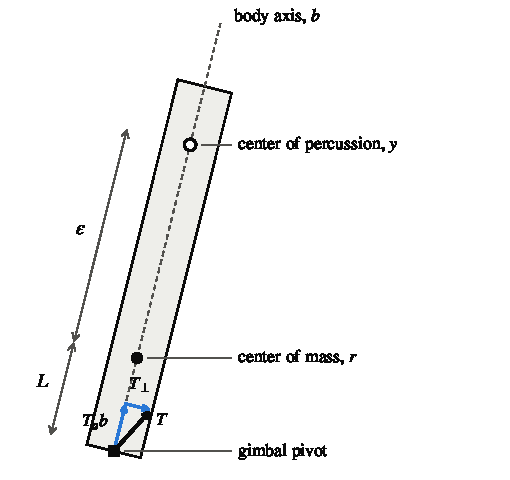
\includegraphics[width=3.4in]{figures/schematic.pdf}
\caption{Vehicle geometry. The gimbal angle is exaggerated.}\label{fig:schematic}
\end{figure}

\begin{table}[t]\centering
\caption{Vehicle and planning parameters}\label{tab:vehicle}
\small
\begin{tabular}{@{}llll@{}}\toprule
Quantity & Value & Quantity & Value \\\midrule
Wet mass, dry mass & 80 kg, 55.9 kg & Thrust range, physical & 400 to 1000 N \\
Transverse inertia $J_t$ (wet) & 63.6 kg\,m$^2$ & Thrust range, planning & 440 to 920 N \\
Pivot to center of mass $L$ (wet) & 0.589 m & Gimbal limit, physical & $\pm15$ deg per axis, 100 deg/s \\
Center-of-percussion offset $\varepsilon$ & 1.35 m & Gimbal limit, planning $\dmax$ & 10 deg cone \\
Specific impulse & 180 s & Tilt limit $\thmax$ & 20 deg \\\bottomrule
\end{tabular}
\end{table}

Deflecting the gimbal produces the torque that turns the body, but it also pushes the center of mass sideways. One point of the
body is not accelerated by that push. Because $\Omega\perp b$, the lateral part of $\ddot b$ is $\Pib\ddot b=\dot\Omega\times b$
with $\Pib=I-bb^{\mathsf T}$, and the second of Eqs.~\eqref{eq:eom} gives $J_t\,\dot\Omega\times b=-LT_\perp$. Hence
\begin{equation}\label{eq:Tperp}
T_\perp=-m\varepsilon\,\Pib\ddot b,\qquad \varepsilon=\frac{J_t}{mL}.
\end{equation}
Substituting Eq.~\eqref{eq:Tperp} into the first of Eqs.~\eqref{eq:eom} and using $\Pib\ddot b=\ddot b+\norm{\dot b}^2b$ shows
that the point $y=r+\varepsilon b$, the center of percussion, obeys
\begin{equation}\label{eq:cop}
\ddot y=\Bigl(\frac{T_a}{m}-\varepsilon\norm{\dot b}^2\Bigr)b-g_0\ez ,
\end{equation}
provided $\varepsilon$ is constant. The lateral thrust does not appear. Seen from $y$, the gimbaled vehicle is a point mass
whose thrust is locked to the body axis. We assume throughout that $\varepsilon$ is constant along the flight. For constant mass
this holds exactly; with depleting mass it requires $J_t$ to scale with $mL$. The mass-property table of the vehicle's
simulator gives $\varepsilon=1.352$, 1.340, and 1.321~m at 79.9, 75, and 70.4~kg, so the assumption is in error by about 1\% over a descent.
The guarantee of Sec.~\ref{sec:proof} is exact for the model with constant $\varepsilon$ and does not extend to that variation;
its effect is measured in Sec.~\ref{sec:results} and is left to feedback.

\section{Limits of an Exact Convex Formulation}\label{sec:imposs}
Let $F$ be the set of initial positions and velocities $(r_0,v_0)$ from which the vehicle can land within its limits at a given
final time. A convex program that receives $(r_0,v_0)$ as LCvx does, through affine constraints, has a feasible set that is
convex jointly in the data and the variables. Its projection onto the data is then convex. If the program were both sound and
complete, that projection would equal $F$, so $F$ would be convex. For 3-DOF descent $F$ is convex, because a thrust direction
that can switch instantly can realize any average of two maneuvers \cite{aumann1965}. For a body that turns at a finite rate it
need not be: with a minimum throttle, the only way to shed vertical impulse is to tilt, and tilting at the limit commits the vehicle
to one direction, so a maneuver that tilts left and its mirror image are both flyable whereas their average is not.

This can be made precise. Consider first the simplest vehicle in which attitude matters: the body axis $b$ turns at a rate
of at most $\omega$, and the thrust per unit mass $a\,d$, with $d$ a unit vector, has $a\ge a_{\min}>0$ and stays within an
angle $\delta$ of $b$. Fix a switch time $s^*$ with $\omega s^*\le\min(\delta,\pi/2-\delta)$. Integrating the equations of
motion twice shows that every trajectory that lands at rest at the origin satisfies
\begin{equation}\label{eq:lam}
r_0+s^*v_0=\int_0^{t_f}(s-s^*)\,a\,d\;\mathrm ds+g_0t_f\Bigl(s^*-\frac{t_f}{2}\Bigr)\ez ,
\end{equation}
and the weight $s-s^*$ changes sign at $s^*$. A body that starts upright is tilted by at most $\omega s$ at time $s$, so by
the triangle inequality on the sphere $d_z\ge\cos(\delta+\omega s)\ge0$ before $s^*$, and $d_z\le1$ after it. The vertical
component of Eq.~\eqref{eq:lam} is therefore largest for a \emph{dive-then-brake} maneuver: tilt at the full rate toward a
horizontal direction $u$ with the thrust deflected fully the same way and the throttle at its minimum until $s^*$, then hold
the attitude and brake with full thrust pointing straight up. A control that attains the same value must also tilt at the
full rate from the first instant, and two body axes tilted by $\omega s$ and $\omega s'$ can lie within the angle
$\omega(s'-s)$ of each other only if they tilt in the same direction; its thrust then has a nonzero horizontal moment along
that direction. The maneuver toward $u$ and its mirror image toward $-u$ both land, and for small $s^*$ both stay above the
ground and inside a glide slope, because the brake decelerates the vehicle throughout. The average of their initial states
has the maximal vertical component of Eq.~\eqref{eq:lam} and zero horizontal component, so no control lands from it. Hence
$F$ is not convex, for any final time. This argument, and its extensions to depleting mass, upright touchdown, and 6-DOF
attitude kinematics, have been checked in the Lean~4 proof assistant \cite{lean4,mathlib,repo}.

For the gimbaled rigid body of Sec.~\ref{sec:model}, in which the deflection that steers the thrust also turns the body, the
same conclusion is proved by computer-assisted certificates at final times of 1 to 5~s under simplifying assumptions
(constant mass and an unlimited gimbal rate) \cite{repo}. On the model and planning limits of this paper, a nonconvex solver
\cite{ipopt} finds landings 1, 2, and 3~m from the launch point of a 4-s hop launched vertically at 6.3~m/s but none on the
launch point itself, which is numerical evidence that the set of reachable landing points has a hole.

The status of the result should be stated exactly. The projection argument is elementary and unconditional. The
nonconvexity of $F$ is proved, and machine-checked, for the simplified model above; for the gimbaled rigid body it is certified
in four special cases and is otherwise an observation, since a solver that finds no landing does not prove that none exists.
This paper does not claim more. Its guarantee (Theorem~\ref{thm:sound}) does not depend on the nonconvexity of $F$, and the
statement that the program cannot be complete (Proposition~\ref{prop:inc}) is conditional on it. What the argument does
establish is that soundness and completeness cannot both be expected, and Eq.~\eqref{eq:cop} makes soundness inexpensive.

\section{A Sound Convex Program}\label{sec:program}
\subsection{Flat Map}
Let $y(t)$ be four times continuously differentiable and define $u=\ddot y+g_0\ez$ and $f=\norm u$. Wherever $u\ne0$, let
\begin{equation}\label{eq:flat}
\begin{gathered}
b=\frac uf,\qquad \dot b=\frac{\Pib\dot u}{f},\qquad \Pib\ddot b=\frac{\Pib\ddot u-2\ip b{\dot u}\,\dot b}{f},\qquad
a=f+\varepsilon\norm{\dot b}^2,\qquad \tau=\sqrt{a^2+\varepsilon^2\norm{\Pib\ddot b}^2},\\
m(t)=m_0\exp\Bigl(-\alpha\int_0^t\tau\,\mathrm dt\Bigr),\qquad T_a=ma,\qquad T_\perp=-m\varepsilon\,\Pib\ddot b,\qquad r=y-\varepsilon b .
\end{gathered}
\end{equation}
The attitude, the body rate, the gimbal angle ($\tan\mu=\varepsilon\norm{\Pib\ddot b}/a$), and the throttle ($\norm T=m\tau$) are
algebraic functions of $y$ and its first four derivatives, and the mass is a quadrature. Section~\ref{sec:proof} shows that
Eqs.~\eqref{eq:flat} are the unique solution of Eqs.~\eqref{eq:eom}. Any sufficiently smooth curve $y$ with $u\ne0$ is
therefore a flight of the vehicle, and only the actuator limits remain to be imposed.

\subsection{Spline Parametrization}
The unknown is $y$, a clamped quintic B-spline with $S$ uniform spans of length $h=t_f/S$. It has $S+5$ coefficients per axis,
63 scalars for $S=16$, and it is four times continuously differentiable, so the gimbal angle and the throttle are continuous.
On each span, $u$, $\dot u$, and $\ddot u$ are polynomials of degree 3, 2, and 1. Raising their B\'ezier control points to
degree 3 gives four \emph{control tuples} $(U^j,U_1^j,U_2^j)$, $j=0,\dots,3$, that are linear in the spline coefficients and satisfy
\begin{equation}\label{eq:hull}
(u,\dot u,\ddot u)(t)=\sum_{j=0}^{3}B_j(t)\,(U^j,U_1^j,U_2^j),\qquad B_j(t)\ge0,\qquad \sum_{j=0}^{3}B_j(t)=1,\qquad \int_{\mathrm{span}}B_j\,\mathrm dt=\frac h4 ,
\end{equation}
where $B_j$ are the cubic Bernstein polynomials of the span. Equation~\eqref{eq:hull} is what allows limits to be enforced at
every instant and not only at grid points \cite{vanloock2015}.

\subsection{The Program}
The data are the current position $r_0$, velocity $v_0$, body axis $b_0$, its rate $\dot b_0$, the lateral angular acceleration
$\beta_0=\Pib\ddot b(0)$ that the present gimbal deflection produces, the mass $m_0$, and the time of flight $t_f$; the target is
the origin. Let $p=\ip U\ez$ for a control tuple, $f_0=\ip{b_0}{u(0)}$, and $\Pi_0=I-b_0b_0^{\mathsf T}$. With auxiliary scalars
$q$, $k$, $G$, and $\sigma$ on each tuple and two constants $\phi>0$ and $\ell_b>0$, the program is
\begin{subequations}\label{eq:prog}
\begin{align}
\text{minimize}\quad & \tfrac h4\textstyle\sum\sigma \label{eq:obj}\\
\text{subject to}\quad & y(0)=r_0+\varepsilon b_0,\quad \dot y(0)=v_0+\varepsilon\dot b_0,\quad u(0)=f_0b_0,\quad \Pi_0\dot u(0)=f_0\dot b_0 \notag\\
& \Pi_0\ddot u(0)=f_0\beta_0+2\ip{b_0}{\dot u(0)}\dot b_0 \label{eq:bc0}\\
& y(t_f)=\varepsilon\ez,\quad \dot y(t_f)=0,\quad u_h(t_f)=\dot u_h(t_f)=\ddot u_h(t_f)=0 \label{eq:bcf}\\
& \norm{U_h}\le\tan\thmax\,p,\qquad p\ge\ell_b,\qquad \norm{U_1}^2\le q\,p \label{eq:tilt}\\
& \norm{U_2-k\ez}+\sin\thmax\,|k|+q\le G,\qquad \varepsilon\,G\le\tan\dmax\,(2\phi p-\phi^2) \label{eq:gimbal}\\
& \bigl\|\bigl(\norm U+\varepsilon q/\ell_b,\ \varepsilon G/\ell_b\bigr)\bigr\|\le\sigma \label{eq:sigma}\\
& p\ge\Tmin\,c_s(z_{lo,s}),\qquad \sigma\le\Tmax\,\tau_s(z_{up,s}) \label{eq:mass}
\end{align}
\end{subequations}
where the subscript $h$ denotes the horizontal part of a vector, Eqs.~(\ref{eq:tilt}--\ref{eq:mass}) hold on every control
tuple, and $s$ indexes spans. The quantities in Eq.~\eqref{eq:mass} bracket the logarithm of the mass:
\begin{equation}\label{eq:z}
z_{up,s}=\ln m_0-\alpha\bigl(\dot y_z(t_s)-\dot y_z(0)+g_0t_s\bigr),\qquad z_{lo,s}=\ln m_0-\alpha\,\tfrac h4\!\!\sum_{\text{spans}\le s}\sum_{j}\sigma^j ,
\end{equation}
with $t_s$ the start of span $s$. Both are affine in the unknowns. The function $c_s$ is the chord of $e^{-z}$ on an interval
to which $z_{lo,s}$ is confined by two further linear constraints, and $\tau_s$ is a tangent of $e^{-z}$; the dry-mass limit is
$z_{lo,S}\ge\ln m_{dry}$. Every constraint is linear or a second-order cone, so Eqs.~\eqref{eq:prog} form an SOCP. The boundary
conditions are linear because $f_0$ and $\ip{b_0}{\dot u(0)}$ are linear in the coefficients, and $(r_0,v_0)$ enter affinely,
exactly as in LCvx.

The reading of the constraints is as follows. Equations~\eqref{eq:bc0} start the plan at the present position, velocity,
attitude, body rate, and gimbal deflection. Equations~\eqref{eq:bcf} end it at rest on the target, upright, without rotation,
and with the gimbal centered. The first of Eqs.~\eqref{eq:tilt} is the tilt limit, and it is exact. The second of
Eqs.~\eqref{eq:gimbal} is the gimbal limit: the snap and the squared jerk of the center-of-percussion path are bounded by the
authority of the gimbal. Equations~\eqref{eq:sigma} and \eqref{eq:mass} are the throttle limits, with the vertical part of $u$
standing in for its magnitude in the lower one. The altitude floor and a glide slope on $r$ are added at sampled instants with
a slack variable, as is usual. The constants are $\phi=7.5$~m/s$^2$, the specific force at which the gimbal constraint is
tightest, and $\ell_b=\Tmin/m_0$. Any positive values keep the guarantee of Sec.~\ref{sec:proof}; they change only how much of
the feasible set is retained.

\section{Soundness}\label{sec:proof}
\begin{theorem}\label{thm:sound}
Assume $\varepsilon$ is constant and $\angle(b_0,\ez)\le\thmax$, and let $y$ be feasible for Eqs.~\eqref{eq:prog}. Then
Eqs.~\eqref{eq:eom}, started from $(r_0,v_0,b_0,\dot b_0,m_0)$ and driven by the thrust $T=T_ab+T_\perp$ of
Eqs.~\eqref{eq:flat}, have the unique solution $r=y-\varepsilon b$, and this solution 1) begins with the lateral thrust the
gimbal is producing, $T_\perp(0)=-m_0\varepsilon\beta_0$; 2) ends with $r=\dot r=0$, $b=\ez$, $\dot b=0$, and $T_\perp=0$;
3) satisfies $\Tmin\le\norm T\le\Tmax$, $\mu\le\dmax$, and $\angle(b,\ez)\le\thmax$ at every $t\in[0,t_f]$; and
4) consumes at most $m_0[1-\exp(-\alpha\tfrac h4\sum\sigma)]$ of propellant.
\end{theorem}
\begin{proof}
\emph{Step 1: the flat map solves the equations of motion.} Differentiating $u=fb$ twice and projecting with $\Pib$ gives
$\Pib\dot u=f\dot b$ and $f\,\Pib\ddot b=\Pib\ddot u-2\dot f\dot b$ with $\dot f=\ip b{\dot u}$, so the quantities named $\dot b$
and $\Pib\ddot b$ in Eqs.~\eqref{eq:flat} are the derivatives of $b$. Take $\Omega=b\times\dot b$. Then $\Omega\perp b$,
$\Omega\times b=\dot b$, and $\dot\Omega=b\times\Pib\ddot b$. The torque of the thrust is $(-Lb)\times T=Lm\varepsilon\,b\times\Pib\ddot b
=J_t\dot\Omega$, because $m\varepsilon L=J_t$. The force is $T-mg_0\ez=m(f+\varepsilon\norm{\dot b}^2)b-m\varepsilon(\ddot b+\norm{\dot b}^2b)-mg_0\ez
=m(\ddot y-\varepsilon\ddot b)=m\ddot r$. Finally $\norm T=m\tau$ and $\dot m=-\alpha\tau m$ by the definition of $m$. The right-hand
sides of Eqs.~\eqref{eq:eom} are locally Lipschitz in the state, so the solution is unique.

\emph{Step 2: boundary conditions.} The end control points of a B\'ezier polygon are values of the curve, so $u_z\ge\ell_b>0$ at
$t=0$ and $t=t_f$. At $t=0$, $u(0)=f_0b_0$ with positive vertical components forces $f_0>0$ and $b(0)=b_0$; the next two
conditions of Eq.~\eqref{eq:bc0} then give $\dot b(0)=\dot b_0$ and $\Pib\ddot b(0)=\beta_0$ by Step~1, and the first two give
$r(0)=r_0$ and $\dot r(0)=v_0$. At $t_f$, $u_h=0$ gives $b=\ez$, then $\dot u_h=0$ gives $\dot b=0$, then $\ddot u_h=0$ gives
$\Pib\ddot b=0$, and $r=y-\varepsilon\ez=0$, $\dot r=\dot y=0$.

\emph{Step 3: pointwise bounds.} Fix an instant and suppose that numbers $q$, $k$, $G$, $\sigma$ satisfy
Eqs.~(\ref{eq:tilt}--\ref{eq:sigma}) with $(U,U_1,U_2)$ replaced by $(u,\dot u,\ddot u)$. Let $p=u_z\le f$. The first of
Eqs.~\eqref{eq:tilt} is $\tan\angle(b,\ez)\le\tan\thmax$. Next, $f\norm{\dot b}^2=\norm{\Pib\dot u}^2/f\le\norm{\dot u}^2/p\le q$.
For the angular acceleration, $f\,\Pib\ddot b=\Pib(\ddot u-k\ez)+k\,\Pib\ez-2\ip b{\dot u}\Pib\dot u/f$. The norm of the first term is at
most $\norm{\ddot u-k\ez}$; $\norm{\Pib\ez}=\sin\angle(b,\ez)\le\sin\thmax$; and
$2|\ip b{\dot u}|\norm{\Pib\dot u}\le\norm{\dot u}^2$ because the two factors are the parts of $\dot u$ along and across $b$. Hence
$f\norm{\Pib\ddot b}\le G$. Since $f^2\ge p^2\ge2\phi p-\phi^2$, the second of Eqs.~\eqref{eq:gimbal} gives
$\varepsilon\norm{\Pib\ddot b}\le\tan\dmax f\le\tan\dmax\,a$, which is $\mu\le\dmax$. Lastly $p\le f\le a\le\tau$, and
$a\le\norm u+\varepsilon q/\ell_b$ and $\varepsilon\norm{\Pib\ddot b}\le\varepsilon G/\ell_b$ because $f\ge p\ge\ell_b$, so
$p\le\tau\le\sigma$ by Eq.~\eqref{eq:sigma}.

\emph{Step 4: every instant.} Equations~(\ref{eq:tilt}--\ref{eq:sigma}) describe a convex set of points $(U,U_1,U_2,q,k,G,\sigma)$
that is the same for the four control tuples of a span. By Eq.~\eqref{eq:hull}, $(u,\dot u,\ddot u)(t)$ together with the
Bernstein-weighted auxiliary numbers is a convex combination of four points of that set, so it lies in the set. Step~3
therefore applies at every instant, with $\sigma(t)=\sum_jB_j(t)\sigma^j$.

\emph{Step 5: mass.} Let $z=\ln m$, so that $\dot z=-\alpha\tau$ and $p\le\tau\le\sigma(t)$. On span $s$,
$z(t)\le z(t_s)\le\ln m_0-\alpha\int_0^{t_s}u_z\,\mathrm dt=z_{up,s}$ and $z(t)\ge z(t_{s+1})\ge\ln m_0-\alpha\int_0^{t_{s+1}}\sigma\,\mathrm dt=z_{lo,s}$,
using the last of Eqs.~\eqref{eq:hull}. Because $e^{-z}$ is decreasing and convex, a chord lies above it and a tangent below it,
so Eq.~\eqref{eq:mass} gives $p(t)\ge\Tmin e^{-z(t)}$ and $\sigma(t)\le\Tmax e^{-z(t)}$, that is,
$\Tmin\le mp\le m\tau=\norm T\le m\sigma\le\Tmax$. The fuel bound is $z(t_f)\ge z_{lo,S}$.
\end{proof}

No relaxation is used, so there is no tightness to establish; this is the difference from LCvx. The price is stated next.

\begin{proposition}\label{prop:inc}
For fixed $b_0$, $\dot b_0$, $\beta_0$, $m_0$, and $t_f$, the set of $(r_0,v_0)$ at which Eqs.~\eqref{eq:prog} are feasible is
convex and is contained in $F$. Whenever $F$ is not convex, the containment is strict.
\end{proposition}
\begin{proof}
The data enter only the right-hand sides of the first two conditions of Eq.~\eqref{eq:bc0}, so the projection argument of
Sec.~\ref{sec:imposs} gives convexity. Containment is Theorem~\ref{thm:sound}. A convex set cannot equal a nonconvex one.
\end{proof}

The program must therefore refuse some landings that exist. The loss has three sources: the lower throttle limit is imposed on
the vertical part of the thrust, so the program never plans to shed thrust by tilting, which is the maneuver the obstruction of
Sec.~\ref{sec:imposs} is built from; the interaction of throttle changes with rotation is bounded, not computed; and control
polygons contain the curves they bound. Section~\ref{sec:results} measures the size of the loss. Two limits are outside the
theorem. The gimbal and throttle slew rates depend on the fifth derivative of $y$ and are not constrained by
Eqs.~\eqref{eq:prog}; they are evaluated exactly on every plan, and a plan that violates them is not flown. The altitude and
glide-slope constraints hold at the sampled instants only.

\section{Guidance Algorithm}\label{sec:algorithm}
The guidance law has three steps. 1) Once, before the descent, the time of flight is set to the smallest $t_f$ at which
Eqs.~\eqref{eq:prog} are feasible, found by bisection in about ten solves, plus a margin of 0.25~s. 2) At every guidance step
the program is solved for the remaining time of flight from the current state estimate. The same program is solved each time;
nothing is carried over from the previous plan, and no initial trajectory, trust region, or penalty weight is required. 3) At
every control step the reference position, velocity, attitude, body rate, throttle, and gimbal angle are evaluated from
Eqs.~\eqref{eq:flat} in closed form and passed to the tracking controller. If a solve is infeasible or its plan fails the
slew-rate check, the final condition $u_z(t_f)=g_0$ (arrival in hover, used by default to soften the touchdown) is dropped, then
the flight time is extended by 0.25, 0.5, or 1.0~s, and otherwise the previous plan, which remains valid, is kept.
Figure~\ref{fig:plan} shows one plan: the vehicle tilts toward the target, tilts back to brake, and arrives upright, with the
thrust rising smoothly from its lower to its upper planning limit.

For $S=16$ the program has 63 spline coefficients. As passed to the solver, with its auxiliary variables, it has about 1000
variables and 480 second-order cones, and one solve takes about 40~ms. The cones are of the types used by 3-DOF LCvx, so
an existing LCvx flight implementation can host the program by changing the constraint builder only; the spline matrices depend
only on $S$ and are computed once.

\begin{figure}[t]\centering
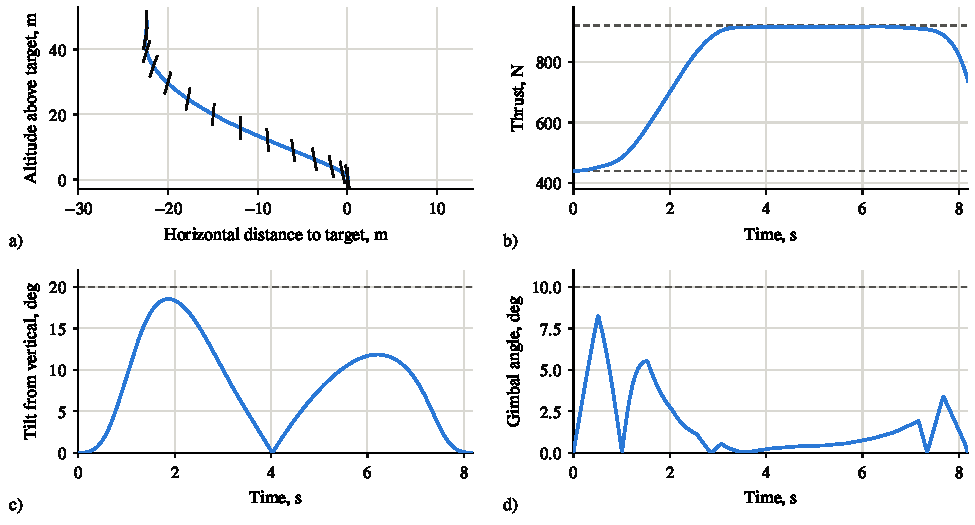
\includegraphics[width=\linewidth]{figures/example_plan.pdf}
\caption{One plan from one solve of Eqs.~\eqref{eq:prog}, a descent from 50 m altitude and 22 m offset: a) path of the center of mass, with the body axis drawn every 0.5 s; b) thrust; c) tilt; and d) gimbal angle. Dashed lines are the planning limits.}\label{fig:plan}
\end{figure}

\section{Results}\label{sec:results}
\subsection{Setup}
All results are numerical and use the vehicle of Table~\ref{tab:vehicle}. The baseline, denoted S, is a standard 6-DOF SCvx
implementation \cite{mao2016,szmuk2018} on the quaternion rigid body with 35 intervals, virtual control, and a trust region; it
uses the same planning limits. The program of Eqs.~\eqref{eq:prog} is denoted F and uses $S=16$. Both are solved with the
Clarabel interior-point solver, and solver times are those it reports on a four-core desktop processor. The simulated plant is
the quaternion rigid body with mass-dependent inertia and lever arm, a $\pm15$~deg gimbal box with a 100~deg/s slew limit, a
400 to 1000~N throttle with a 2000~N/s slew limit, wind of up to 3~m/s with gusts, 2\% thrust noise, a 5\% error in specific
impulse, and gimbal misalignment. One tracking controller, a linear-quadratic regulator in center-of-percussion coordinates
running at 50~Hz, is used for both planners. A landing is counted as successful if the touchdown speed is at most 1~m/s, the
lateral error at most 1~m, and the tilt at most 5~deg. The test set is 40 in-air descents (initial altitude 40 to 60~m, offset
up to 21~m, initial tilt up to 3~deg) and 30 hops launched from the pad at 5 to 6~m/s toward a point up to 4~m away. The final
time for S is 0.5~s above the minimum final time found for an attitude-aware iterative planner from our earlier work \cite{repo}. For
reference, the 3-DOF LCvx guidance currently used on the vehicle, which plans thrust directions the body cannot follow, landed
11 of the 40 in-air cases and none of the hops in the same tests.

\subsection{Open-Loop Comparison}
Table~\ref{tab:open} compares single plans on eight in-air scenarios at equal final time. At a fixed final time the fuel is
nearly the same for any planner, because the boundary conditions fix the total impulse; F uses 0.10\% more on average. The
difference is the work: one SOCP against 25 to 35. Program~\eqref{eq:prog} needs a slightly longer flight at the limit, which
is the incompleteness of Proposition~\ref{prop:inc}.

\begin{table}[t]\centering
\caption{Single plans on eight in-air scenarios}\label{tab:open}
\small
\begin{tabular}{@{}lcc@{}}\toprule
 & S (successive convexification) & F (this work) \\\midrule
Convex programs per plan & 25 to 35 & 1 \\
Solver time per plan, median, s & 1.30 & 0.046 \\
Fuel at equal final time, relative to S & reference & $+0.10\%$ mean, $+0.28\%$ maximum \\
Minimum feasible final time, s & reference\textsuperscript{a} & $+0.04$ to $+0.22$ \\
Open-loop replay error, planner's own model & 2 nm to 10 $\mu$m & at most 23 nm \\
Open-loop replay error, plant mass table, median, m & 0.45 & 0.03 \\\bottomrule
\multicolumn{3}{@{}l}{\footnotesize\textsuperscript{a}Minimum certified final time of the iterative planner of Ref.~\cite{repo}, at which S also converges.}
\end{tabular}
\end{table}

\subsection{Exactness, Model Error, and Soundness}
To test Step~1 of the proof, the throttle and gimbal commands of F were applied without feedback to the quaternion rigid body
with depleting mass and constant $\varepsilon$, integrated to a relative tolerance of $10^{-13}$. In 16 replays, half of them
starting tilted by 3~deg and rotating, the vehicle came to rest within 23~nm and 12~nm/s of the target, which is integration
error. Each planner is exact in its own model. S freezes $J_t$ and $L$ at their initial values, which lets $J_t/(mL)$ drift by
6\% over a descent, whereas the plant keeps it within 1\%. Replayed without feedback against the plant's mass table, plans of S
miss by a median of 0.45~m and plans of F by 0.03~m.

To test Theorem~\ref{thm:sound}, 300 random problems, wider than the test set, were each solved with the constants above and
with randomly chosen ones. Of the 600 solves, 458 were feasible, and none of the plans violated a planning limit at any of 1201
instants. To test Proposition~\ref{prop:inc}, both planners and a nonconvex solver \cite{ipopt} were run on a grid of 20 hops
of exactly 4~s (launch speeds of 5 to 7~m/s, landing offsets of 0 to 6~m). No flyable plan was found for 11 of the targets, and
F is infeasible at all 11. It is also infeasible at five of the nine targets where a plan exists, which it reaches with 0.06 to
0.41~s more flight time. A 3-DOF LCvx program reports an optimal solution at all 20 targets.

\subsection{Closed Loop with Computation Time Counted}
Simulation studies of guidance commonly apply each plan at the instant its state was sampled. Here a plan computed from the state
at time $t$ becomes active at $t$ plus its solver time, and each planner replans as soon as it can: S at most every 0.5~s and F
every 0.1~s. F chooses its own time of flight as in Sec.~\ref{sec:algorithm}. Table~\ref{tab:closed} and Fig.~\ref{fig:td} give
the results. Both planners land every case. F is more accurate laterally by more than an order of magnitude, touches down more
slowly, and moves the gimbal a third as far. On hops it uses 5\% more fuel, because it flies them 0.1~s longer on average and
extended the flight during a replan in six runs. With every solver time multiplied by four, to represent a slower flight
computer, S fails four of the 30 hops, and F, replanning every 0.2~s, fails none.

\begin{table}[t]\centering
\caption{Closed-loop results with each plan applied after its solver time (median / 95th percentile / maximum)}\label{tab:closed}
\small\setlength{\tabcolsep}{4.5pt}
\begin{tabular}{@{}lcccc@{}}\toprule
 & \multicolumn{2}{c}{In-air descents (40 runs)} & \multicolumn{2}{c}{Pad hops (30 runs)} \\\cmidrule(lr){2-3}\cmidrule(l){4-5}
 & S & F & S & F \\\midrule
Successful landings & 40 & 40 & 30 & 30 \\
Lateral error, cm & 5.9 / 15.7 / 18.3 & 0.2 / 0.8 / 1.1 & 3.9 / 7.6 / 8.2 & 0.4 / 1.4 / 2.0 \\
Touchdown speed, m/s & 0.23 / 0.46 / 0.58 & 0.19 / 0.28 / 0.29 & 0.54 / 0.81 / 0.88 & 0.14 / 0.22 / 0.23 \\
Tilt at touchdown, deg & 0.21 / 0.70 / 1.23 & 0.11 / 0.30 / 0.63 & 0.96 / 2.46 / 2.54 & 0.20 / 0.62 / 0.87 \\
Fuel, mean, kg & 3.58 & 3.52 & 1.46 & 1.54 \\
Solver time per replan, s (mean / maximum) & 1.05 / 4.9 & 0.031 / 0.39 & 0.35 / 2.4 & 0.017 / 0.052 \\
Convex programs per plan, mean & 20.2 & 1.4 & 12.7 & 1.1 \\
Gimbal travel per flight, mean, deg & 156 & 45 & 182 & 62 \\\bottomrule
\end{tabular}
\end{table}

\begin{figure}[t]\centering
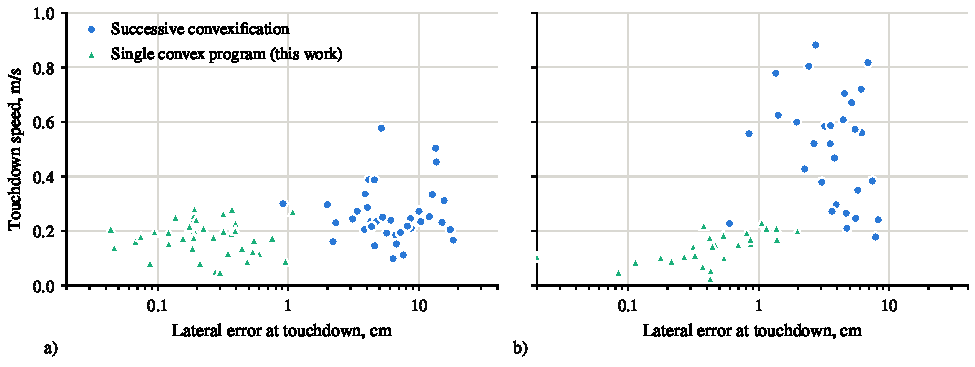
\includegraphics[width=\linewidth]{figures/touchdown.pdf}
\caption{Touchdown accuracy with computation time counted: a) 40 in-air descents and b) 30 pad hops.}\label{fig:td}
\end{figure}

The mechanism behind this advantage is the cost of a plan. A plan of F is as good as a plan of S: when both planners are
artificially given the same 1-Hz replanning rate, zero computation delay, and the same final time, the lateral accuracy is the
same, a median of 3.1~cm for each in the air and 2.4~cm for each on hops (F then still touches down more slowly on hops, 0.23
against 0.51~m/s, and never needs to extend the final time in the air, which S does in 32 of 40 runs). What F adds is that a
plan costs 30~ms instead of 1~s, so the vehicle is corrected five to ten times as often from a state that is tens of
milliseconds old instead of a second old. That is the accuracy in Table~\ref{tab:closed}, and it is the relevant comparison
for a flight computer, where computation is never free. The margin widens as the processor slows, as the fourfold test shows:
the iterative planner runs out of time first. Giving S the arrival-in-hover condition does not change this
(hops: 0.52~m/s and 4.0~cm).

\subsection{Limitations}
F is worse than S in three respects: fuel on short hops, the minimum flight time (by up to 0.4~s on 4-s hops), and, when S is
given zero computation time, the touchdown speed in the air (S is lower in 27 of 40 cases). The slew-rate limits are outside
Theorem~\ref{thm:sound}; fewer than 1\% of replans failed the check and were not flown. The worst replan took 0.39~s, when every
fallback was tried, and a flight implementation should bound that chain. Theorem~\ref{thm:sound} is proved here and tested
numerically but is not machine-checked, apart from Eq.~\eqref{eq:cop}, which is machine-checked for constant mass \cite{repo}. The assumption of constant
$\varepsilon$ must be confirmed from measured mass properties, and a guarantee that tolerates a bounded variation of
$\varepsilon$ is not available. Nothing here has been run on flight hardware, with actuator lag, or
with state-estimation error, and the SCvx baseline was not retuned or reimplemented for speed. The proof of
Theorem~\ref{thm:sound} and the experiments have not been reproduced independently; the software, its tests, the result
files, and the scripts that regenerate each table are public for that purpose \cite{repo}.

\section{Conclusion}
This paper gave a conservative single-SOCP planner for a gimbaled-lander model, with guarantees on thrust magnitude, gimbal
angle, and tilt that hold at every instant. Writing the problem for the center of percussion removes the coupling between
steering and translation, makes the dynamics linear, and leaves the actuator limits as the only nonconvex part; restricting
those limits, instead of relaxing them, yields one second-order cone program whose feasible points satisfy the model and the
three limits by proof. The guarantee is for a constant center-of-percussion offset and does not cover slew rates or path
constraints between samples. The program is conservative: on the cases studied it costs a tenth of a percent of fuel and a few
tenths of a second of minimum flight time, and a convex program of this kind cannot be expected to be exact. Its practical
value is its speed and its lack of tuning. It has no initial guess, trust region, or iteration count, and it solves fast enough
to replan at the rate of the control system. That speed is what produced the order-of-magnitude gain in touchdown accuracy over successive
convexification in our simulations, and it matters most where computation is scarce: on a processor four times slower the
iterative planner began to fail landings and this one did not. Future work is to extend the guarantee to a varying
center-of-percussion offset and to slew rates, to bound the loss of feasible landings, to formalize the proof, to have the
results reproduced independently, and to fly it.

\section*{Acknowledgments}
% AIAA policy (Ethical Standards, Sec. 3) requires a description of AI use here and a disclosure at submission.
% The first two sentences below are a factual description of how this work was produced. Complete the third truthfully.
An artificial-intelligence system (Claude, Anthropic) was used extensively in this work. It derived and wrote the proofs,
wrote the planning and simulation software, ran the numerical experiments, and drafted the text and figures of this
manuscript. [State here what the Contributing Student Authors did themselves, for example: defined the problem and the
vehicle data, directed the investigation, and checked the derivations, the code, and the results. State any other
contributors and sponsors.] The authors are responsible for the content of the paper.

\begin{thebibliography}{99}
\bibitem{acikmese2007} A\c{c}{\i}kme\c{s}e, B., and Ploen, S. R., ``Convex Programming Approach to Powered Descent Guidance for Mars
Landing,'' \emph{Journal of Guidance, Control, and Dynamics}, Vol.~30, No.~5, 2007, pp.~1353--1366. \url{https://doi.org/10.2514/1.27553}.
\bibitem{acikmese2011} A\c{c}{\i}kme\c{s}e, B., and Blackmore, L., ``Lossless Convexification of a Class of Optimal Control Problems
with Non-Convex Control Constraints,'' \emph{Automatica}, Vol.~47, No.~2, 2011, pp.~341--347. \url{https://doi.org/10.1016/j.automatica.2010.10.037}.
\bibitem{acikmese2013} A\c{c}{\i}kme\c{s}e, B., Carson, J. M., and Blackmore, L., ``Lossless Convexification of Nonconvex Control Bound
and Pointing Constraints of the Soft Landing Optimal Control Problem,'' \emph{IEEE Transactions on Control Systems Technology},
Vol.~21, No.~6, 2013, pp.~2104--2113. \url{https://doi.org/10.1109/TCST.2012.2237346}.
\bibitem{malyuta2022} Malyuta, D., Reynolds, T. P., Szmuk, M., Lew, T., Bonalli, R., Pavone, M., and A\c{c}{\i}kme\c{s}e, B., ``Convex
Optimization for Trajectory Generation: A Tutorial on Generating Dynamically Feasible Trajectories Reliably and Efficiently,''
\emph{IEEE Control Systems Magazine}, Vol.~42, No.~5, 2022, pp.~40--113. \url{https://doi.org/10.1109/MCS.2022.3187542}.
\bibitem{mao2016} Mao, Y., Szmuk, M., and A\c{c}{\i}kme\c{s}e, B., ``Successive Convexification of Non-Convex Optimal Control Problems
and Its Convergence Properties,'' \emph{2016 IEEE 55th Conference on Decision and Control}, IEEE, 2016, pp.~3636--3641.
\url{https://doi.org/10.1109/CDC.2016.7798816}.
\bibitem{szmuk2018} Szmuk, M., and A\c{c}{\i}kme\c{s}e, B., ``Successive Convexification for 6-DoF Mars Rocket Powered Landing with
Free-Final-Time,'' AIAA Paper 2018-0617, Jan. 2018. \url{https://doi.org/10.2514/6.2018-0617}.
\bibitem{szmuk2020} Szmuk, M., Reynolds, T. P., and A\c{c}{\i}kme\c{s}e, B., ``Successive Convexification for Real-Time
Six-Degree-of-Freedom Powered Descent Guidance with State-Triggered Constraints,'' \emph{Journal of Guidance, Control, and
Dynamics}, Vol.~43, No.~8, 2020, pp.~1399--1413. \url{https://doi.org/10.2514/1.G004549}.
\bibitem{fliess1995} Fliess, M., L\'evine, J., Martin, P., and Rouchon, P., ``Flatness and Defect of Non-Linear Systems: Introductory
Theory and Examples,'' \emph{International Journal of Control}, Vol.~61, No.~6, 1995, pp.~1327--1361. \url{https://doi.org/10.1080/00207179508921959}.
\bibitem{martin1996} Martin, P., Devasia, S., and Paden, B., ``A Different Look at Output Tracking: Control of a VTOL Aircraft,''
\emph{Automatica}, Vol.~32, No.~1, 1996, pp.~101--107. \url{https://doi.org/10.1016/0005-1098(95)00099-2}.
\bibitem{mellinger2011} Mellinger, D., and Kumar, V., ``Minimum Snap Trajectory Generation and Control for Quadrotors,''
\emph{2011 IEEE International Conference on Robotics and Automation}, IEEE, 2011, pp.~2520--2525. \url{https://doi.org/10.1109/ICRA.2011.5980409}.
\bibitem{desiderio2013} Desiderio, D., and Lovera, M., ``Guidance and Control for Planetary Landing: Flatness-Based Approach,''
\emph{IEEE Transactions on Control Systems Technology}, Vol.~21, No.~4, 2013, pp.~1280--1294. \url{https://doi.org/10.1109/TCST.2012.2202664}.
\bibitem{vanloock2015} Van Loock, W., Pipeleers, G., and Swevers, J., ``Optimal Motion Planning for Differentially Flat Systems with
Guaranteed Constraint Satisfaction,'' \emph{2015 American Control Conference}, IEEE, 2015, pp.~4245--4250. \url{https://doi.org/10.1109/ACC.2015.7171996}.
\bibitem{wang2026} Wang, C., and Chen, Z., ``B-Spline-Based Convex Programming for Fuel-Optimal Powered Descent Guidance,''
\emph{Advances in Space Research}, Vol.~78, No.~4, 2026, pp.~3919--3934. \url{https://doi.org/10.1016/j.asr.2026.06.014}.
\bibitem{freire2023} Freire, V., and Xu, X., ``Flatness-Based Quadcopter Trajectory Planning and Tracking with Continuous-Time
Safety Guarantees,'' \emph{IEEE Transactions on Control Systems Technology}, Vol.~31, No.~6, 2023, pp.~2319--2334.
\url{https://doi.org/10.1109/TCST.2023.3250954}.
\bibitem{aumann1965} Aumann, R. J., ``Integrals of Set-Valued Functions,'' \emph{Journal of Mathematical Analysis and Applications},
Vol.~12, No.~1, 1965, pp.~1--12. \url{https://doi.org/10.1016/0022-247X(65)90049-1}.
\bibitem{lean4} de Moura, L., and Ullrich, S., ``The Lean 4 Theorem Prover and Programming Language,'' \emph{Automated Deduction --
CADE 28}, Lecture Notes in Computer Science, Vol.~12699, Springer, Cham, 2021, pp.~625--635. \url{https://doi.org/10.1007/978-3-030-79876-5_37}.
\bibitem{mathlib} The mathlib Community, ``The Lean Mathematical Library,'' \emph{Proceedings of the 9th ACM SIGPLAN International
Conference on Certified Programs and Proofs}, ACM, New York, 2020, pp.~367--381. \url{https://doi.org/10.1145/3372885.3373824}.
\bibitem{repo} Propulsive Landers at Georgia Tech, ``lossless-navigation-paper: Lean Proofs, Certificates, and Guidance Software for
Powered Descent,'' software and data repository, 2026. \url{https://github.com/Propulsive-Landers-GT/lossless-navigation-paper}.
\bibitem{ipopt} W\"achter, A., and Biegler, L. T., ``On the Implementation of an Interior-Point Filter Line-Search Algorithm for
Large-Scale Nonlinear Programming,'' \emph{Mathematical Programming}, Vol.~106, No.~1, 2006, pp.~25--57. \url{https://doi.org/10.1007/s10107-004-0559-y}.
\end{thebibliography}
\end{document}
